% Pixel coordinates (bp at the source resolution) clip the two stored FDS
% panels and their common colour ramp without resampling the fields.
\begingroup
\newcommand{\matchedrow}[2]{\noindent\makebox[.095\linewidth][l]{\small\sffamily #1}%
  \raisebox{-.5\height}{#2}\par}
\newcommand{\fieldpair}[4]{%
  \matchedrow{OP-1}{\includegraphics[viewport=96 180 996 284,clip,width=.905\linewidth]{../previews/#1}}\vspace{3pt}
  \matchedrow{OP-6}{\includegraphics[viewport=96 67 996 171,clip,width=.905\linewidth]{../previews/#1}}\vspace{4pt}
  \noindent\hspace*{.095\linewidth}\makebox[.905\linewidth][c]{%
    \makebox[4em][r]{\small #2}\hspace{4pt}%
    \includegraphics[viewport=419 28 659 42,clip,width=.21\linewidth]{../previews/#1}%
    \hspace{4pt}\makebox[4em][l]{\small #3}}\par
  \matchedcaption{#4}}
\newcommand{\matchedcaption}[1]{\vspace{4pt}{\raggedright\fontsize{10bp}{12bp}\selectfont\itshape #1\par}}
\fieldpair{OP1_OP6_temperature_matched.png}{20}{$\geq$870\,$^{\circ}$C}{\tempCaption}
\vspace{14pt}
\fieldpair{OP1_OP6_extinction_matched.png}{0}{$\geq$0.10\,m$^{-1}$}{\smokeCaption}
\vspace{14pt}
\matchedrow{OP-1}{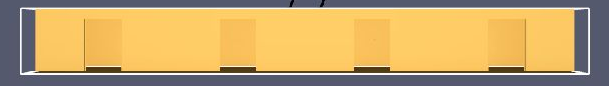
\includegraphics[width=.905\linewidth]{../previews/OP1_1p12_side_elevation.png}}\vspace{3pt}
\matchedrow{OP-6}{
\includegraphics[width=.905\linewidth]{../previews/OP6_1p12_side_elevation.png}}
\matchedcaption{\modelCaption}
\endgroup